\section{Introducción} % (fold)
\label{sec:introducción}
	Se ha desarrollado una aplicación Liberty basada en Python, con los siguientes cinco servicios:
	\begin{itemize}
		\item Language Translator
		\item Visual Recognition
		\item Test to Speech
		\item Natural Language Understanding
		\item Cloudant NoSQL DB
	\end{itemize}
	El objetivo de la aplicación es ofrecer un servicio de análisis de imágenes y de frases en diferentes idiomas.

	\todo{meter una foto de la aplicación entera junto con el historial (aunque no salga el historial en el resto de fotos da igual)}
% section introducción (end)

\section{Capturas de pantalla de la aplicación} % (fold)
\label{sec:capturas_de_pantalla_de_la_aplicación}
\newpage
\clearpage
\subsection{Responsividad} % (fold)
\label{sub:responsividad}

% subsection responsividad (end)
\begin{figure}[htp!]
    \centering
    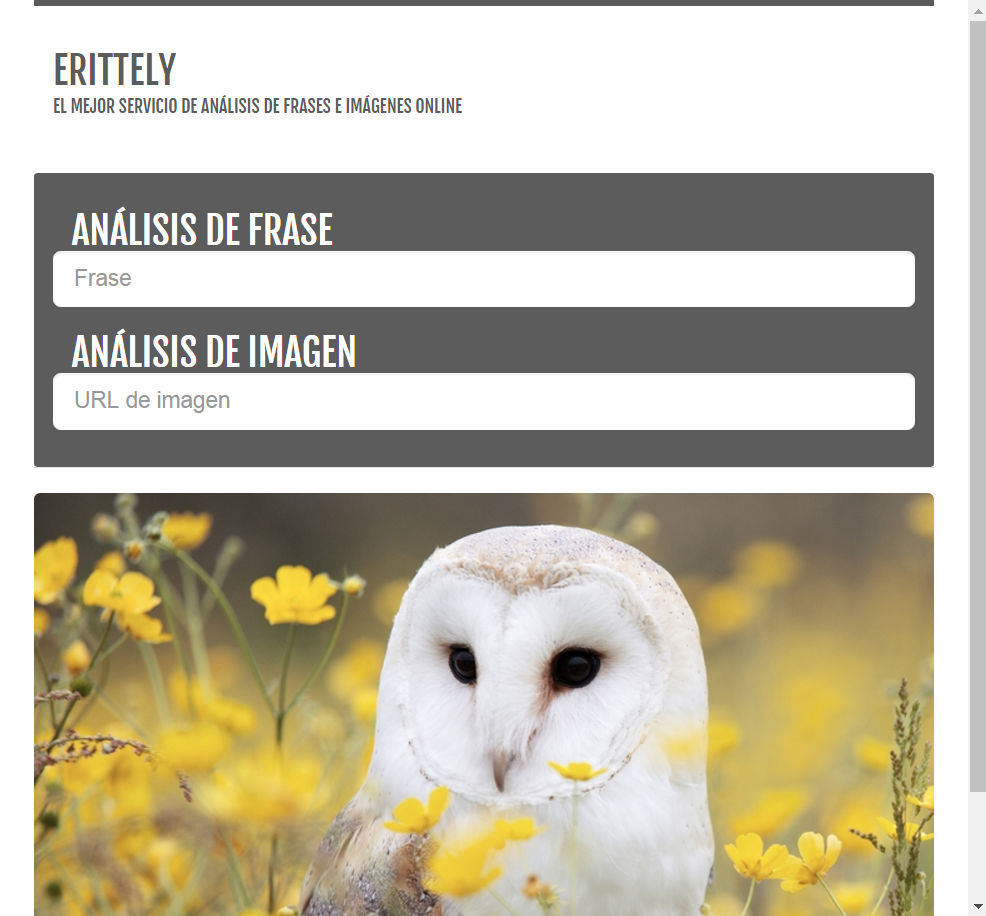
\includegraphics[width=\textwidth]{images/1}
    \caption{Pantalla de inicio de la aplicación}
    \label{fig:1}
\end{figure}
\begin{figure}[htp!]
    \centering
    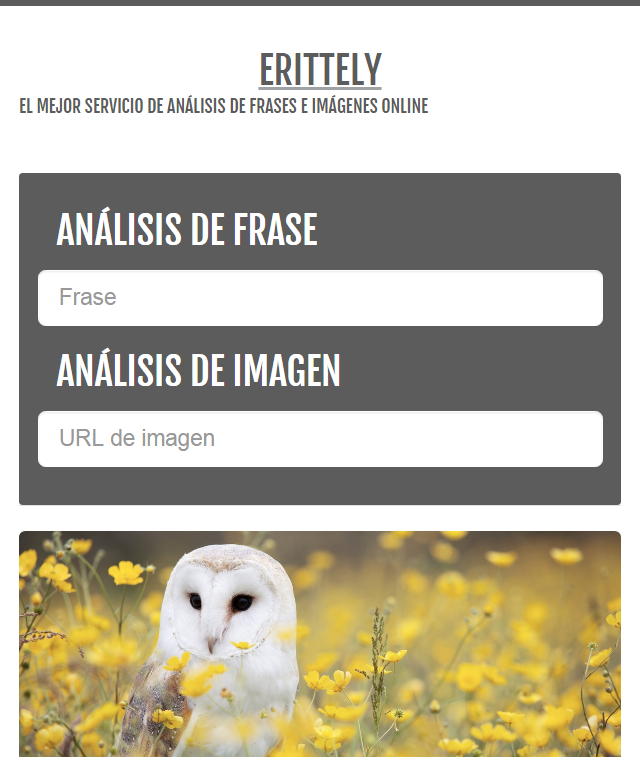
\includegraphics[width=\textwidth]{images/2}
    \caption{Pantalla de inicio de la aplicación mostrando la responsividad (I)}
    \label{fig:2}
\end{figure}
\begin{figure}[htp!]
    \centering
    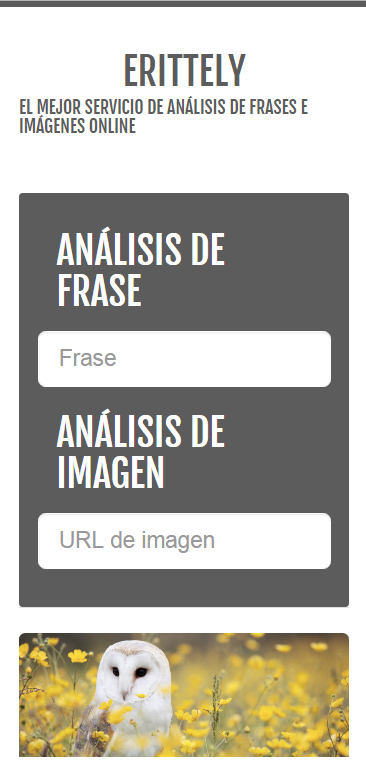
\includegraphics[width=\textwidth]{images/3}
    \caption{Pantalla de inicio de la aplicación mostrando la responsividad (II)}
    \label{fig:3}
\end{figure}
\begin{figure}[htp!]
    \centering
    \includegraphics[width=\textwidth]{images/4}
    \caption{Pantalla de inicio de la aplicación mostrando la responsividad (III)}
    \label{fig:4}
\end{figure}
\newpage
\clearpage
\subsection{Funcionamiento de la aplicación} % (fold)
\label{sub:funcionamiento_de_la_aplicación}

% subsection funcionamiento_de_la_aplicación (end)
\begin{figure}[htp!]
    \centering
    \includegraphics[width=\textwidth]{images/5}
    \caption{Ejemplo de funcionamiento de la aplicación (I)}
    \label{fig:5}
\end{figure}
\begin{figure}[htp!]
    \centering
    \includegraphics[width=\textwidth]{images/6}
    \caption{Ejemplo de funcionamiento de la aplicación (II)}
    \label{fig:6}
\end{figure}
\begin{figure}[htp!]
    \centering
    \includegraphics[width=\textwidth]{images/7}
    \caption{Ejemplo de funcionamiento de la aplicación (III)}
    \label{fig:7}
\end{figure}
\begin{figure}[htp!]
    \centering
    \includegraphics[width=\textwidth]{images/9}
    \caption{Otro ejemplo de funcionamiento de la aplicación (I)}
    \label{fig:9}
\end{figure}
\begin{figure}[htp!]
    \centering
    \includegraphics[width=\textwidth]{images/10}
    \caption{Otro ejemplo de funcionamiento de la aplicación (II)}
    \label{fig:10}
\end{figure}
\begin{figure}[htp!]
    \centering
    \includegraphics[width=\textwidth]{images/11}
    \caption{Otro ejemplo de funcionamiento de la aplicación (III)}
    \label{fig:11}
\end{figure}
% section capturas_de_pantalla_de_la_aplicación (end)